\documentclass[crop,tikz,10pt]{standalone}
\usepackage{tikz}
	\usetikzlibrary{shapes}
	\usetikzlibrary{automata}
	\usetikzlibrary{arrows}
	\usetikzlibrary{backgrounds}
	\usetikzlibrary{calc}
	\usetikzlibrary{positioning}
	\usetikzlibrary{patterns}
	\usetikzlibrary{shadows}
	\usetikzlibrary{shadings}
	\usetikzlibrary{decorations.pathmorphing}
	\usetikzlibrary{decorations.pathreplacing}

\usepackage[scaled]{helvet}
\renewcommand{\familydefault}{\sfdefault}

\usepackage{siunitx}
\usepackage[version=4]{mhchem}

\usepackage{xcolor}
\definecolor{TUMBlue}{HTML}{0065BD}
\definecolor{TUMBlueDarker}{HTML}{003359}



\input{../../../../../resources/latex/_symbols.qmd}


\newcommand{\apsize}{\fontsize{44pt}{20pt}\selectfont}
\newcommand{\mpsize}{\fontsize{48pt}{20pt}\selectfont}
\newcommand{\ompsize}{\fontsize{35pt}{20pt}\selectfont}
\newcommand{\mycell}[2]{\begin{tabular}{c}\ce{#1}\\\SI{#2}{\percent}\end{tabular}}

\begin{document}


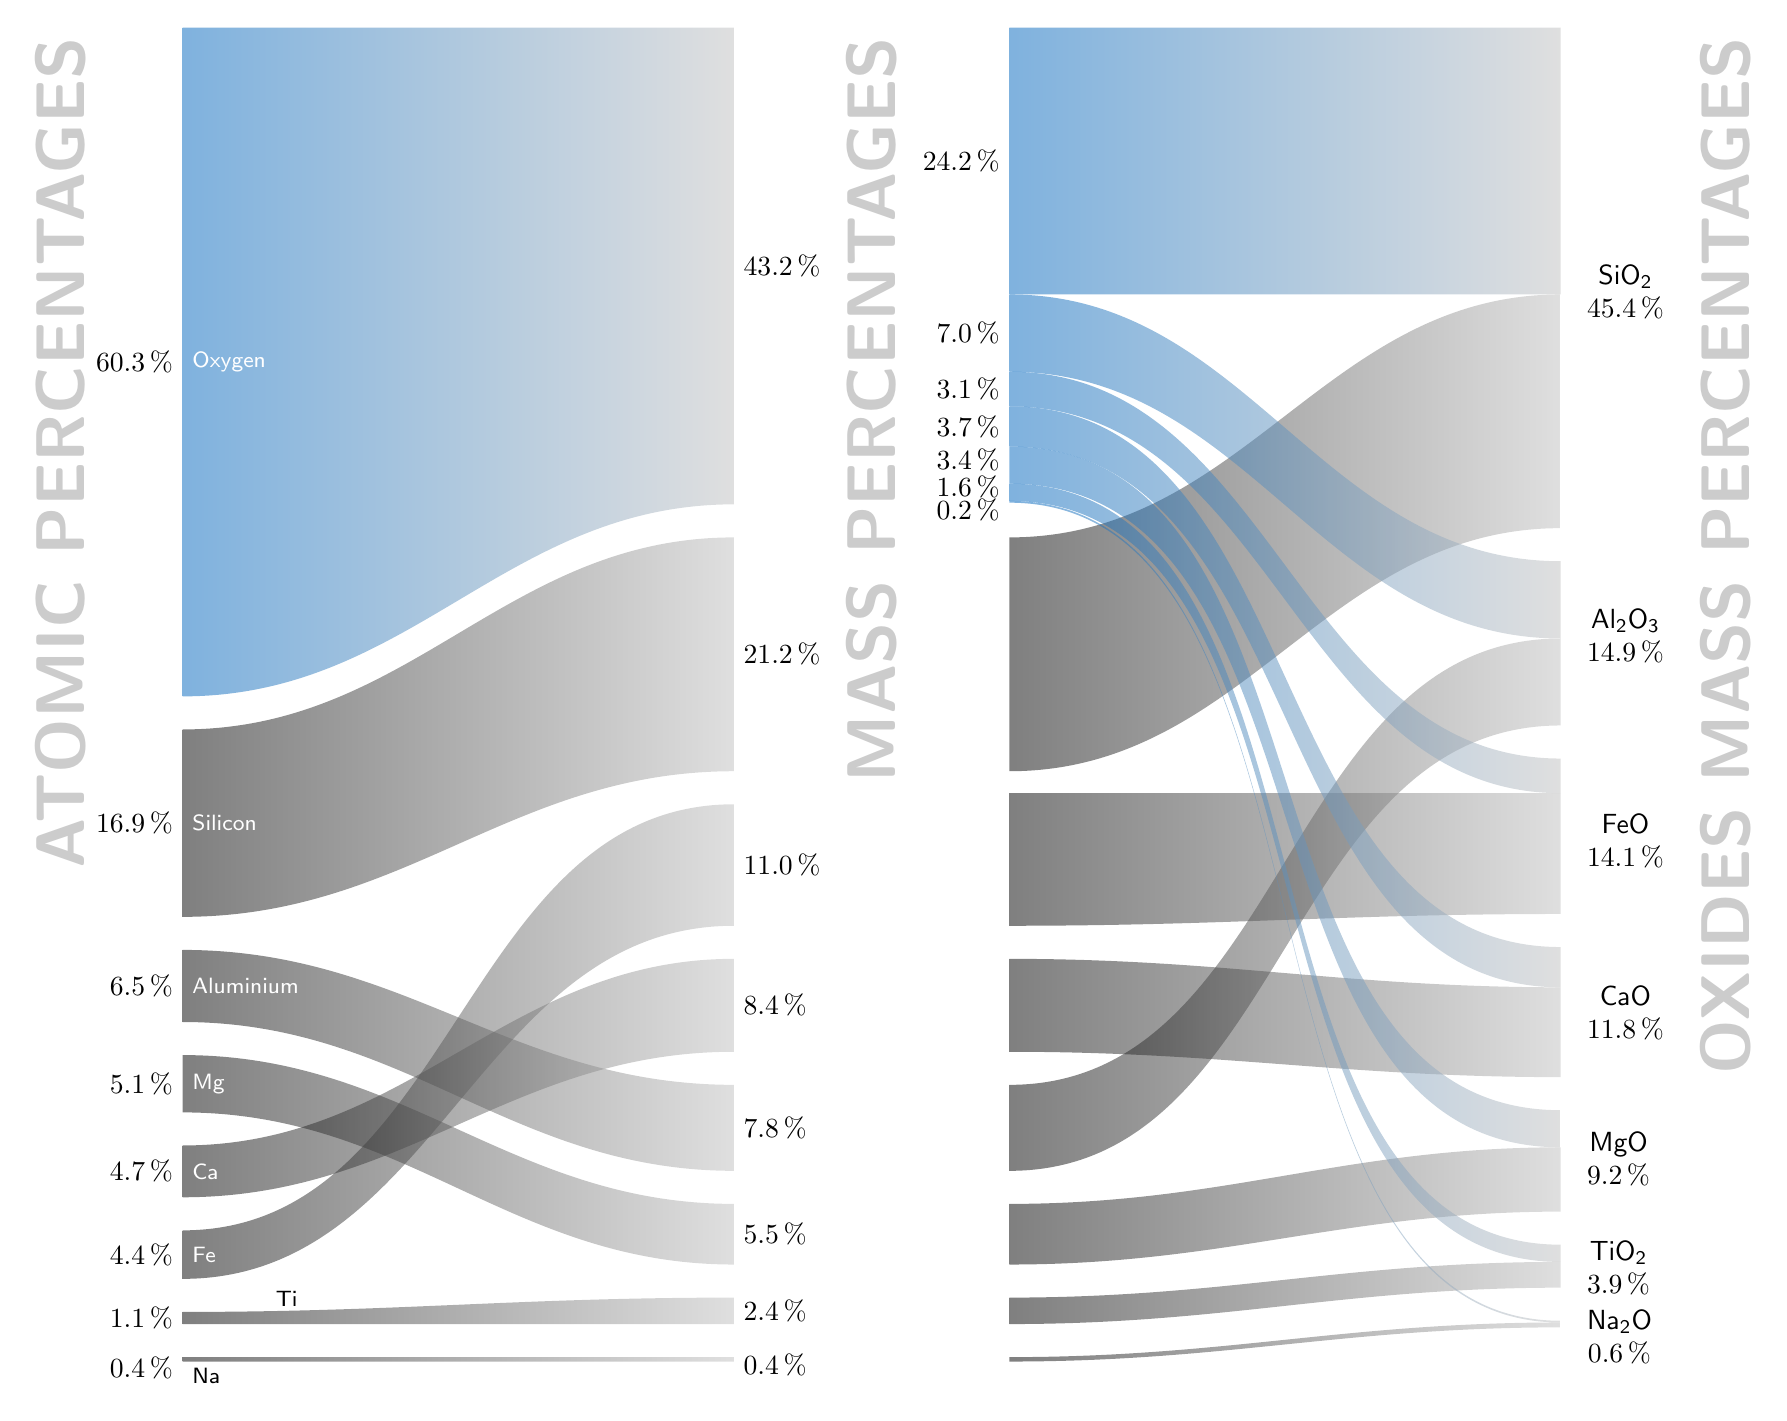
\begin{tikzpicture}[scale=1.4,
    main/.style={draw=none, left color=black, right color=lightgray, fill opacity=0.5},
    nmain/.style={text=black, fill opacity=1},
    nel/.style={text=white, fill opacity=1, font=\footnotesize},
]

    \def\d{5}
    \def\m{2.5}
    \def\a{0.3}

    % background
    \node[rotate=90, font=\apsize\bf, fill opacity=0.2, anchor=south east] at (-0.8, 0) {ATOMIC PERCENTAGES};
    \node[rotate=90, font=\mpsize\bf, fill opacity=0.2, anchor=east] at ($(\d, 0) + (1.25,0)$) {MASS PERCENTAGES};
    \node[rotate=90, font=\ompsize\bf, fill opacity=0.2, anchor=east] at ($(2*\d+\m, 0) + (1.5,0)$) {OXIDES MASS PERCENTAGES};


    % O 60.3% (1) >> 43.2% (1)
    \draw[main, left color=TUMBlue] (0, 0.0)     to[in=180, out=0] 
                (\d, 0.0)    -- node[nmain,right] {\SI{43.2}{\percent}}
                (\d, -4.324) to[in=0, out=180] 
                (0, -6.066)  -- node[nel, right] {Oxygen} node[nmain,left] {\SI{60.3}{\percent}} cycle;

    % Si 16.9% (2) >> 21.2% (2)
    \draw[main] ($(0, -6.066)  - (0, \a)$) to[in=180, out=0] 
                ($(\d, -4.324) - (0, \a)$) -- node[nmain,right] {\SI{21.2}{\percent}}
                ($(\d, -6.445) - (0, \a)$) to[in=0, out=180] 
                ($(0, -7.766)  - (0, \a)$) -- node[nel, right] {Silicon} node[nmain,left] {\SI{16.9}{\percent}} cycle;

    
    % Al 6.5% (3) >> 7.8% (5)
    \draw[main] ($(0, -7.766) - (0, 2*\a)$) to[in=180, out=0] 
                ($(\d, -8.39) - (0, 4*\a)$) -- node[nmain,right] {\SI{7.8}{\percent}}
                ($(\d, -9.17) - (0, 4*\a)$) to[in=0, out=180] 
                ($(0, -8.42)  - (0, 2*\a)$) -- node[nel, right] {Aluminium} node[nmain,left] {\SI{6.5}{\percent}} cycle;
                              
    
    % Mg 5.1% (4) >> 5.5% (6)
    \draw[main] ($(0, -8.42)   - (0, 3*\a)$) to[in=180, out=0] 
                ($(\d, -9.17)  - (0, 5*\a)$) -- node[nmain,right] {\SI{5.5}{\percent}}
                ($(\d, -9.72)  - (0, 5*\a)$) to[in=0, out=180] 
                ($(0, -8.94)   - (0, 3*\a)$) -- node[nel, right] {Mg} node[nmain,left] {\SI{5.1}{\percent}} cycle;
                              
    % Ca 4.7% (5) >> 8.4% (4)
    \draw[main] ($(0, -8.94)   - (0, 4*\a)$) to[in=180, out=0] 
                ($(\d, -7.547) - (0, 3*\a)$) -- node[nmain,right] {\SI{8.4}{\percent}}
                ($(\d, -8.39)  - (0, 3*\a)$) to[in=0, out=180] 
                ($(0, -9.41)   - (0, 4*\a)$) -- node[nel, right] {Ca} node[nmain,left] {\SI{4.7}{\percent}} cycle;
    
    % Fe 4.4% (6) >> 11.0% (3)
    \draw[main] ($(0, -9.41)   - (0, 5*\a)$) to[in=180, out=0] 
                ($(\d, -6.445) - (0, 2*\a)$) -- node[nmain,right] {\SI{11.0}{\percent}}
                ($(\d, -7.547) - (0, 2*\a)$) to[in=0, out=180] 
                ($(0, -9.85)   - (0, 5*\a)$) -- node[nel, right] {Fe} node[nmain,left] {\SI{4.4}{\percent}} cycle;

    % Ti 1.1% (7) >> 2.4% (7)
    \draw[main] ($(0, -9.85)  - (0, 6*\a)$) to[in=180, out=0] 
                ($(\d, -9.72) - (0, 6*\a)$) -- node[nmain,right] {\SI{2.4}{\percent}}
                ($(\d, -9.96) - (0, 6*\a)$) to[in=0, out=180] 
                ($(0, -9.96)  - (0, 6*\a)$) -- node[nel, right, black, xshift=30px, yshift=7px] {Ti} node[nmain,left] {\SI{1.1}{\percent}} cycle;

    % Na 0.4% (8) >> 0.4% (8)
    \draw[main] ($(0, -9.96)  - (0, 7*\a)$) to[in=180, out=0] 
                ($(\d, -9.96) - (0, 7*\a)$) -- node[nmain,right, yshift=-2px] {\SI{0.4}{\percent}}
                ($(\d, -10.0) - (0, 7*\a)$) to[in=0, out=180] 
                ($(0, -10.0)  - (0, 7*\a)$) -- node[nel, right, black, yshift=-6px] {Na} node[nmain,left, yshift=-3px] {\SI{0.4}{\percent}} cycle;
    


    %::. MINERALS
    % SiO2 45.4% >> 24.2% O
    \draw[main, left color=TUMBlue] ($(\d+\m, 0.0)$)     to[in=180, out=0]
                ($(2*\d+\m, 0.0)$)   -- 
                ($(2*\d+\m, -2.42)$) to[in=0, out=180]
                ($(\d+\m, -2.42)$)   -- node[nmain,left] {\SI{24.2}{\percent}} cycle;

    \draw[main] ($(\d+\m, -4.324)  - (0, \a)$) to[in=180, out=0] node[nmain,right,at end] {\mycell{SiO2}{45.4}}
                ($(2*\d+\m, -2.42)$)           -- 
                ($(2*\d+\m, -4.54)$)            to[in=0, out=180]
                ($(\d+\m, -6.445)  - (0, \a)$) -- cycle;
                
    % Al2O3 14.9% >> 7.01% O
    \draw[main, left color=TUMBlue] ($(\d+\m, -2.42)$)              to[in=180, out=0]
                ($(2*\d+\m, -4.54)  - (0, \a)$) -- 
                ($(2*\d+\m, -5.241) - (0,\a)$)  to[in=0, out=180]
                ($(\d+\m, -3.121)$)             --  node[nmain,left] {\SI{7.0}{\percent}} cycle;

    \draw[main] ($(\d+\m, -8.39)    - (0, 4*\a)$) to[in=180, out=0] node[nmain,right,at end] {\mycell{Al2O3}{14.9}}
                ($(2*\d+\m, -5.241) - (0, \a)$)   -- 
                ($(2*\d+\m, -6.03)  - (0,\a)$)    to[in=0, out=180]
                ($(\d+\m, -9.17)    - (0, 4*\a)$) -- cycle;
                
    % FeO 14.1% >> 3.14% O
    \draw[main, left color=TUMBlue] ($(\d+\m, -3.121)$)               to[in=180, out=0]
                ($(2*\d+\m, -6.03)  - (0, 2*\a)$) -- 
                ($(2*\d+\m, -6.344) - (0, 2*\a)$) to[in=0, out=180]
                ($(\d+\m, -3.435)$)               --  node[nmain,left] {\SI{3.1}{\percent}} cycle;

    \draw[main] ($(\d+\m, -6.344)    - (0, 2*\a)$)  to[in=180, out=0] node[nmain,right,at end,yshift=-18px] {\mycell{FeO}{14.1}}
                ($(2*\d+\m, -6.344) - (0, 2*\a)$)  -- 
                ($(2*\d+\m, -7.44)    - (0, 2*\a)$) to[in=0, out=180]
                ($(\d+\m, -7.547)    - (0, 2*\a)$)  -- cycle;

    % CaO 11.8% >> 3.652% O
    \draw[main, left color=TUMBlue] ($(\d+\m, -3.435)$)                to[in=180, out=0]
                ($(2*\d+\m, -7.44)   - (0, 3*\a)$) -- 
                ($(2*\d+\m, -7.8052) - (0, 3*\a)$) to[in=0, out=180]
                ($(\d+\m, -3.8002)$)               --  node[nmain,left] {\SI{3.7}{\percent}} cycle;

    \draw[main] ($(\d+\m, -7.547)    - (0, 3*\a)$)  to[in=180, out=0] node[nmain,right,at end,yshift=-10px] {\mycell{CaO}{11.8}}
                ($(2*\d+\m, -7.8052) - (0, 3*\a)$)  -- 
                ($(2*\d+\m, -8.62)   - (0, 3*\a)$)  to[in=0, out=180]
                ($(\d+\m, -8.39)     - (0, 3*\a)$)  -- cycle;

    % MgO 9.2% >> 3.367% O
    \draw[main, left color=TUMBlue] ($(\d+\m, -3.8002)$)                to[in=180, out=0]
                ($(2*\d+\m, -8.62)   - (0, 4*\a)$) -- 
                ($(2*\d+\m, -8.9567) - (0, 4*\a)$) to[in=0, out=180]
                ($(\d+\m, -4.1369)$)               --  node[nmain,left,yshift=2px] {\SI{3.4}{\percent}} cycle;

    \draw[main] ($(\d+\m, -9.17)     - (0, 5*\a)$)  to[in=180, out=0] node[nmain,right,at end,yshift=-5px] {\mycell{MgO}{9.2}}
                ($(2*\d+\m, -8.9567) - (0, 4*\a)$)  -- 
                ($(2*\d+\m, -9.54)   - (0, 4*\a)$)  to[in=0, out=180]
                ($(\d+\m, -9.72)     - (0, 5*\a)$)  -- cycle;

    % TiO2 3.9% >> 1.562% O
    \draw[main, left color=TUMBlue] ($(\d+\m, -4.1369)$)                to[in=180, out=0, looseness=0.95]
                ($(2*\d+\m, -9.54)    - (0, 5*\a)$) -- 
                ($(2*\d+\m, -9.6962)  - (0, 5*\a)$) to[in=0, out=180, looseness=0.95]
                ($(\d+\m, -4.2931)$)                --  node[nmain,left,yshift=2px] {\SI{1.6}{\percent}} cycle;

    \draw[main] ($(\d+\m, -9.72)     - (0, 6*\a)$)  to[in=180, out=0] node[nmain,right,at end,yshift=-3px] {\mycell{TiO2}{3.9}}
                ($(2*\d+\m, -9.6962) - (0, 5*\a)$)  -- 
                ($(2*\d+\m, -9.93)   - (0, 5*\a)$)  to[in=0, out=180]
                ($(\d+\m, -9.96)     - (0, 6*\a)$)  -- cycle;

    % Na2O 0.6% >> 0.1549% O
    \draw[main, left color=TUMBlue] ($(\d+\m, -4.2931)$)               to[in=180, out=0, looseness=0.9]
                ($(2*\d+\m, -9.93)   - (0, 6*\a)$) -- 
                ($(2*\d+\m, -9.9455) - (0, 6*\a)$) to[in=0, out=180, looseness=0.9]
                ($(\d+\m, -4.309)$)                --  node[nmain,left,yshift=-3px] {\SI{0.2}{\percent}} cycle;

    \draw[main] ($(\d+\m, -9.96)     - (0, 7*\a)$) to[in=180, out=0] node[nmain,right,at end,yshift=-6px] {\mycell{Na2O}{0.6}}
                ($(2*\d+\m, -9.9455) - (0, 6*\a)$) -- 
                ($(2*\d+\m, -9.99)   - (0, 6*\a)$) to[in=0, out=180]
                ($(\d+\m, -10.0)     - (0, 7*\a)$) -- cycle;

\end{tikzpicture}

\end{document}